\section{I-Measure}
We have already known that the Venn diagrams can give us a clear picture of the relations among sets. In order to construct  similar information diagrams to facilitate our analysis of information, we need to introduce a method to connect Shannon's information measure with things in set theory. We introduce a few basic concepts in measure theory which will be used subsequently. These concepts will be illustrated by simple examples.\\

\begin{definition}[Field]\label{field}
The field $\mathcal{F}_{n}$ generated by sets $\tilde{X}_{1}, \tilde{X}_{2}, \cdots, \tilde{X}_{n}$ is the collection of sets which can be obtained by any sequence of usual set operations (union, intersection, complement, and difference) on $\tilde{X}_{1}, \tilde{X}_{2}, \cdots, \tilde{X}_{n}$\\
\end{definition}

\begin{definition}[Atom]\label{atom}
The atoms of $\mathcal{F}_{n}$ are sets of the form $\cap_{i=1}^{n} Y_{i},$ where $Y_{i}$ is either$\tilde{X}_{i}$ or $\tilde{X}_{i}^{c},$ the complement of $\tilde{X}_{i}$\\
\end{definition}

\begin{definition}[Signed Measure]\label{sm}
A real function $\mu$ defined on $\mathcal{F}_{n}$ is called a signed measure if it is set-additive, i.e., for disjoint $A$ and $B$ in $\mathcal{F}_{n}$
\begin{equation}
\mu(A \cup B)=\mu(A)+\mu(B)
\end{equation}
\end{definition}

For a signed measure $\mu,$ we have
\begin{equation}
\mu(\emptyset)=0
\end{equation}
which can be seen as follows. For any $A$ in $\mathcal{F}_{n}$
\begin{equation}
\mu(A)=\mu(A \cup \emptyset)=\mu(A)+\mu(\emptyset)
\end{equation}
by set-additivity because $A$ and $\emptyset$ are disjoint. A signed measure $\mu$ on $\mathcal{F}_{n}$ is completely specified by its values on the atoms of $\mathcal{F}_{n} .$ The values of $\mu$ on the other sets in $\mathcal{F}_{n}$ can be obtained via set-additivity.

Until now, we have found a practical method to measure a set. We'll see how we can introduce a measure for the information in section \ref{sec2.1}.


\begin{figure}[ht]
 
\centering
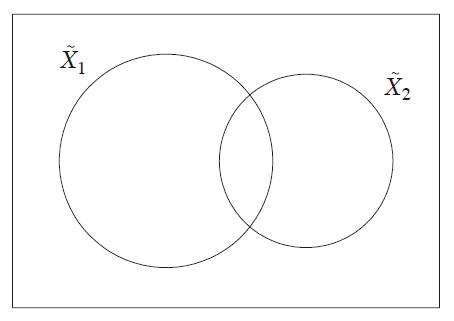
\includegraphics[scale=0.4]{tex/Im1.png}
\caption{The Venn diagram for $\tilde{X}_{1}$ and $\tilde{X}_{2}$}
\label{im1}
 
\end{figure}

\subsection{I-Measure between 2 R.V.s}
\label{sec2.1}

To start with, we first formulate the one-to-one correspondence
between Shannon's information measures and set theory for two random variables. For random variables ${X}_1$ and ${X}_2$, let $\tilde{X}_{1}$ and $\tilde{X}_{2}$ be sets respectively corresponding to ${X}_1$ and ${X}_2$. The sets $\tilde{X}_{1}$ and $\tilde{X}_{2}$ generates the field $\mathcal{F}_{n}$ whose
atoms are 

$$\tilde{X}_{1} \cap \tilde{X}_{2}, \tilde{X}_{1}^{c} \cap \tilde{X}_{2}, \tilde{X}_{1} \cap \tilde{X}_{2}^{c}, \tilde{X}_{1}^{c} \cap \tilde{X}_{2}^{c}$$
Their relationship is shown by a Venn diagram in Figure \ref{im1}.

  In our formulation, we set the universal set $\Omega$ to $\tilde{X}_{1} \cup \tilde{X}_{2}$. With this choice of $\Omega,$ the Venn diagram for $\tilde{X}_{1}$ and $\tilde{X}_{2}$ is represented by the diagram in Figure \ref{im2}. For simplicity, the sets $\tilde{X}_{1}$ and $\tilde{X}_{2}$ are respectively labeled by $X_{1}$ and $X_{2}$ in the diagram. We call this the information diagram for the random variables $X_{1}$ and $X_{2} .$ In this diagram, the universal set, which is the union of $\tilde{X}_{1}$ and $\tilde{X}_{2}$ is not shown explicitly just as in a usual Venn diagram. Note that with our choice of the universal set, the atom $\tilde{X}_{1}^{c} \cap \tilde{X}_{2}^{c}$ degenerates to the empty set.
  
\begin{figure}[ht]
 
\centering
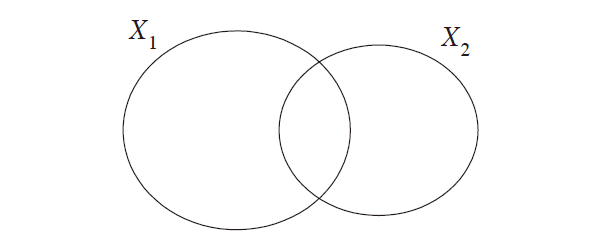
\includegraphics[scale=0.4]{tex/Im2.png}
\caption{The information diagram for ${X}_{1}$ and
${X}_{2}$}
\label{im2}
 
\end{figure}

From what we know about random variables $X_{1}$ and $X_{2}$, we can explicit the Shannon's information measures
\[
H\left(X_{1}\right), H\left(X_{2}\right), H\left(X_{1} | X_{2}\right), H\left(X_{2} | X_{1}\right), H\left(X_{1}, X_{2}\right), I\left(X_{1} ; X_{2}\right)
\]
Writing $A \cap B^{c}$ as $A-B,$ we now define a signed measure $\mu^{*}$ by
\begin{equation}
    \mu^{*}\left(\tilde{X}_{1}-\tilde{X}_{2}\right)=H\left(X_{1} | X_{2}\right)
\end{equation}
\begin{equation}
\mu^{*}\left(\tilde{X}_{2}-\tilde{X}_{1}\right)=H\left(X_{2} | X_{1}\right)
\end{equation}
and
\begin{equation}
\mu^{*}\left(\tilde{X}_{1} \cap \tilde{X}_{2}\right)=I\left(X_{1} ; X_{2}\right)
\end{equation}
These are the values of $\mu^{*}$ on the nonempty atoms of $\mathcal{F}_{2}$ (i.e., atoms of $\mathcal{F}_{2}$ other $\left.\operatorname{than} \tilde{X}_{1}^{c} \cap \tilde{X}_{2}^{c}\right) .$ The values of $\mu^{*}$ on the other sets on $\mathcal{F}_{2}$ can be obtained via set-additivity. In particular, we can easily formulate these following relations
\begin{equation}
\mu^{*}\left(\tilde{X}_{1} \cup \tilde{X}_{2}\right) =H\left(X_{1}, X_{2}\right)
\end{equation}

\begin{equation}
\mu^{*}\left(\tilde{X}_{1}\right) =H\left(X_{1}\right)
\end{equation}

and
\begin{equation}
\mu^{*}\left(\tilde{X}_{2}\right)=H\left(X_{2}\right)
\end{equation}



For example, $\mu^{*}\left(\tilde{X}_{1} \cup \tilde{X}_{2}\right)$ can be calculated by
\begin{align}
&\mu^{*}\left(\tilde{X}_{1} \cup \tilde{X}_{2}\right)\\
&=\mu^{*}\left(\tilde{X}_{1}-\tilde{X}_{2}\right)+\mu^{*}\left(\tilde{X}_{2}-\tilde{X}_{1}\right)+\mu^{*}\left(\tilde{X}_{1} \cap \tilde{X}_{2}\right)\\
&=H\left(X_{1} | X_{2}\right)+H\left(X_{2} | X_{1}\right)+I\left(X_{1} ; X_{2}\right) \\
&=H\left(X_{1}, X_{2}\right) 
\end{align}


By now, the relationship between Shannon's information measures and signed measure (i.e. the set theory) is clear for 2 R.V.s. By the approach of sign mapping, we can change between Shannon's information measures into signed measure, and vice versa. 



 \subsection{\protect\boldmath Construction of  \texorpdfstring{$\mu^{*}$}{\textmu*}}
 
 In this section, we are finding a more general conclusion, which means to find a similar relation in a higher random variable space. For n $\geq$ 2, consider n random variables ${X}_{1}$;${X}_{2}$; ... ;${X}_{n}$. For any random variable X,
let $\tilde{X}$ be a set corresponding to X. Let
\begin{equation}
    \mathcal{N}_{n}=\{1,2, \cdots, n\}
\end{equation}
Define the universal set $\Omega$ to be the union of the sets$\tilde{X}_{1}, \tilde{X}_{2}, \cdots, \tilde{X}_{n},$ i.e.
\begin{equation}
    \Omega=\bigcup_{i \in \mathcal{N}_{n}} \tilde{X}_{i}
\end{equation}
And we use $\mathcal{F}_{n}$ to denote the field generated by $\tilde{X}_{1}, \tilde{X}_{2}, \cdots, \tilde{X}_{n} .$\\

The set
\[
A_{0}=\bigcap_{i \in \mathcal{N}_{n}} \tilde{X}_{i}^{c}
\]   
is called the empty atom of $\mathcal{F}_{n}$ because

\begin{equation}
    \bigcap_{i \in \mathcal{N}_{n}} \tilde{X}_{i}^{c}=\left(\bigcup_{i \in \mathcal{N}_{n}} \tilde{X}_{i}\right)^{c}=\Omega^{c}=\emptyset
\end{equation}


All the atoms of $\mathcal{F}_{n}$ other than $A_{0}$ are called nonempty atoms.\\
 
 To simplify notation, we will use $X_{G}$ to denote $\left(X_{i}, i \in G\right)$ and $\tilde{X}_{G}$ to denote $\cup_{i \in G} \tilde{X}_{i}$ for any nonempty subset $G$ of $\mathcal{N}_{n}$\\
 

\begin{theorem}\label{th1}
Let
\begin{equation}
    \mathcal{B}=\left\{\tilde{X}_{G}: G \text { is a nonempty subset of } \mathcal{N}_{n}\right\}
\end{equation}
Then a signed measure $\mu$ on $\mathcal{F}_{n}$ is completely specified by $\{\mu(B), B \in \mathcal{B}\}$
which can be any set of real numbers.
\end{theorem}
When introducing our work of "PI-Measure", we will use a similar way as this proof to show a connection in $\mu^{*}$ and decomposed mutual information, and that proof will be given.


Until now the work to expand signed measures into higher space is finished. Next we'll look at how to substitute signed measures into Shannon's information measure when n $\geq$ 2.\\

We now construct the I-Measure $\mu^{*}$ on $\mathcal{F}_{n}$ using Theorem \ref{th1} by defining%%%%%%%%%%%%%
\begin{equation}
    \mu^{*}\left(\tilde{X}_{G}\right)=H\left(X_{G}\right)
\end{equation}
for all nonempty subsets $G$ of $\mathcal{N}_{n} .$ In order for $\mu^{*}$ to be meaningful, it has to be consistent with all Shannon's information measures. In that case, the following must hold for all (not necessarily disjoint $)$ subsets $G, G^{\prime}, G^{\prime \prime}$ of $\mathcal{N}_{n}$ where $G$ and $G^{\prime}$ are nonempty:
\begin{equation}\label{eqx1}
    \mu^{*}\left(\tilde{X}_{G} \cap \tilde{X}_{G^{\prime}}-\tilde{X}_{G^{\prime \prime}}\right)=I\left(X_{G} ; X_{G^{\prime}} | X_{G^{\prime \prime}}\right)
\end{equation}
When $G^{\prime \prime}=\emptyset,(\ref{eqx1})$ becomes
\begin{equation}
\mu^{*}\left(\tilde{X}_{G} \cap \tilde{X}_{G^{\prime}}\right)=I\left(X_{G} ; X_{G^{\prime}}\right)
\end{equation}
When $G=G^{\prime},(\ref{eqx1})$ becomes
\begin{equation}
\mu^{*}\left(\tilde{X}_{G}-\tilde{X}_{G^{\prime \prime}}\right)=H\left(X_{G} | X_{G^{\prime \prime}}\right)
\end{equation}
When $G=G^{\prime}$ and $G^{\prime \prime}=\emptyset,(\ref{eqx1})$ becomes
\begin{equation}
    \mu^{*}\left(\tilde{X}_{G}\right)=H\left(X_{G}\right)
\end{equation}

From these cases we know that (\ref{eqx1}) can cover all the 4 conditions that Shannon's information measure may have. Thus, we can say that Equation (\ref{eqx1}) holds, if and only if $\mu^{*}$ is consistent with all Shannon's information measures.

\begin{theorem} $\mu^{*}$ is the unique signed measure on $\mathcal{F}_{n}$ which is consistent with all Shannon's information measures.
\end{theorem}

Proof. Consider
\[
\begin{array}{l}
\mu^{*}\left(\tilde{X}_{G} \cap \tilde{X}_{G^{\prime}}-\tilde{X}_{G^{\prime \prime}}\right) \\
=\mu^{*}\left(\tilde{X}_{G \cup G^{\prime \prime}}\right)+\mu^{*}\left(\tilde{X}_{G^{\prime} \cup G^{\prime \prime}}\right)-\mu^{*}\left(\tilde{X}_{G \cup G^{\prime} \cup G^{\prime \prime}}\right)-\mu^{*}\left(\tilde{X}_{G^{\prime \prime}}\right) \\
=H\left(X_{G \cup G^{\prime \prime}}\right)+H\left(X_{G^{\prime} \cup G^{\prime \prime}}\right)-H\left(X_{G \cup G^{\prime} \cup G^{\prime \prime}}\right)-H\left(X_{G^{\prime \prime}}\right) \\
=I\left(X_{G} ; X_{G^{\prime}} | X_{G^{\prime \prime}}\right)
\end{array}
\]
i.e., $\mu^{*}$ is consistent with all Shannon's information measures. In order that $\mu^{*}$ is consistent with all Shannon's information measures, for all nonempty subsets $G$ of $\mathcal{N}_{n}, \mu^{*}$ has to satisfy Equation (\ref{eqx1}), which in fact is the definition of $\mu^{*}$. Therefore, $\mu^{*}$ is the unique signed measure on $\mathcal{F}_{n}$ which is consistent with all Shannon's information measures.

 \subsection{Markov Chain, a Special Case}
\label{sec:markov}
 
 
 
All the contents above together, give us the possibility to draw a clear picture of the relationship among Shannon's information measure of discrete random variables. (The n = 3 case is shown below)
\begin{figure}[ht]
 
\centering
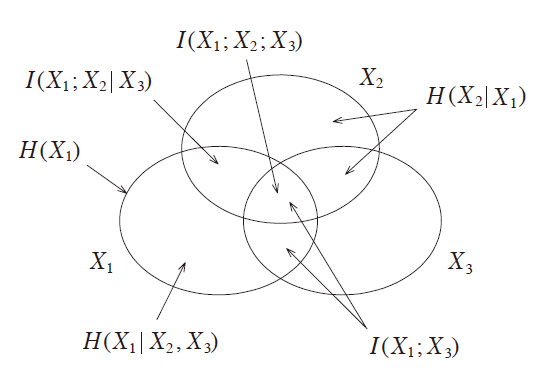
\includegraphics[scale=0.4]{tex/Im3.png}
\caption{The information diagram for ${X}_{1}$, ${X}_{2}$ and ${X}_{3}$}
\label{im3}
 
\end{figure}


In this section, we'll focus on a special case of this relation, i.e. the Markov Chain (MC). We explore the structure of Shannon's information measures when $X_{1} \rightarrow X_{2} \rightarrow \cdots \rightarrow X_{n}$ forms a Markov chain. To start with, we consider $n=3,$ i.e., $X_{1} \rightarrow X_{2} \rightarrow X_{3}$ forms a Markov chain. since
\[
\mu^{*}\left(\tilde{X}_{1} \cap \tilde{X}_{2}^{c} \cap \tilde{X}_{3}\right)=I\left(X_{1} ; X_{3} | X_{2}\right)=0
\]
the atom $\tilde{X}_{1} \cap \tilde{X}_{2}^{c} \cap \tilde{X}_{3}$ does not have to be displayed in an information diagram. Therefore, in constructing the information diagram, the regions representing the random variables $X_{1}, X_{2},$ and $X_{3}$ should overlap with each other such that the region corresponding to the atom $\tilde{X}_{1} \cap \tilde{X}_{2}^{c} \cap \tilde{X}_{3}$ is empty, while the regions corresponding to all other nonempty atoms are nonempty. Figure 3.7 shows such a construction, in which each random variable is represented by a "mountain." From Figure 3.7, we see that $\tilde{X}_{1} \cap \tilde{X}_{2} \cap \tilde{X}_{3},$ as the only atom on which $\mu^{*}$ may take a negative value, now becomes identical to the atom $\tilde{X}_{1} \cap \tilde{X}_{3} .$ Therefore, we have
\[
\begin{aligned}
I\left(X_{1} ; X_{2} ; X_{3}\right) &=\mu^{*}\left(\tilde{X}_{1} \cap \tilde{X}_{2} \cap \tilde{X}_{3}\right) \\
&=\mu^{*}\left(\tilde{X}_{1} \cap \tilde{X}_{3}\right) \\
&=I\left(X_{1} ; X_{3}\right) \\
& \geq 0
\end{aligned}
\]
%%%%%%%%%%%%%%%%%%%
%%%%%%%%%%%%%%%%%%%%%%%%%%%%%%%%%%%%%%
%%%%%%%%%%%%%%%%%%%%%%%%%%%%%%%%%%%%%%
%%%%%%%%%%%%%%%%%%%%%%%%%%%%%%%%%%%%%%
%%%%%%%%%%%%%%%%%%%%%%%%%%%%%%%%%%%%%%




 Information Diagrams for Zero Measure
In Markov Chain $X_{1} \rightarrow X_{2} \rightarrow X_{3}$, since \begin{equation}\mu^{*}\left(\tilde{X}_{1} \cap \tilde{X}_{2}^{c} \cap \tilde{X}_{3}\right)=I\left(X_{1} ; X_{3} | X_{2}\right)=0\end{equation}
        We don't have to plot that region out in the information diagram, making the diagram simpler and more useful when reasoning about Shannon information measures. And for MC with 4 or more R.V.s, we can also find out that some parts needn't to be plotted, because of the properties of Markov Chain.


Above all, we've introduced several general ideas in constructing the correspondence between set theory and Shannon information. These ideas will be revisited later , helping us find a correspondence between another type of information measure and set theory.

